\documentclass{article}
\usepackage{graphicx}
\usepackage[margin=1.5cm]{geometry}
\usepackage{amsmath}

\begin{document}

\title{Warm Up Exercises: Unit 3, Forces}
\author{Prof. Jordan C. Hanson}

\maketitle

\section{Memory Bank}

\begin{enumerate}
\item $\vec{F} = m \vec{a}$ ... Newton's 2nd Law
\item $N_x = mg \sin\theta$, $N_y = mg \cos\theta$ ... Components of normal force on an inclined plane.
\end{enumerate}

\begin{figure}[ht]
\centering
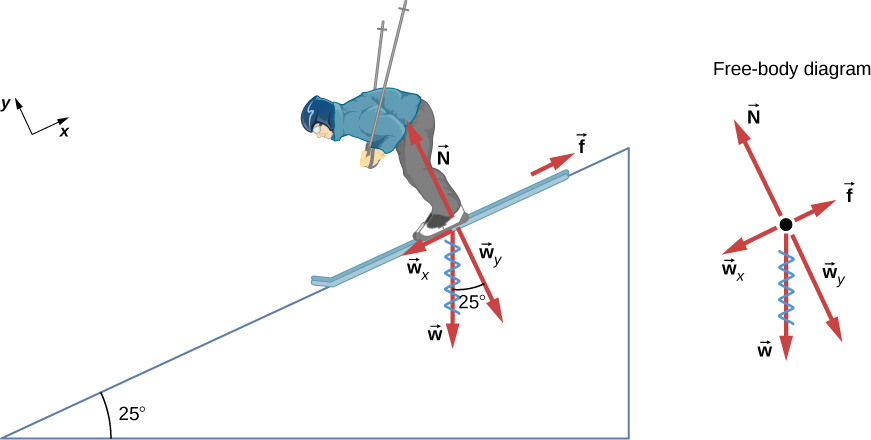
\includegraphics[width=0.5\textwidth]{figures/ski.jpeg}
\caption{\label{fig:1} Skiing on an incline, and the forces involved.}
\end{figure}

\section{Chapter 5 - Forces}

\begin{enumerate}
\item Consider the skier on the slope in Fig. \ref{fig:1}. Her mass including equipment is 60.0 kg. (a) What is her acceleration if friction is negligible? (b) What is her acceleration if friction is 45.0 N? (c) What would the friction force have to be to stop the skier from moving?
\end{enumerate}

\end{document}
